We present a construction for pegged ledgers
%over a generic epoch-based PoS blockchain
that is based
on Ouroboros PoS~\cite{C:KRDO17}, but also applicable to other PoS
systems such as Snow White~\cite{DBLP:journals/iacr/BentovPS16a}
and Algorand~\cite{algorand}.
Our protocol
will implement a system of ledgers with pegging %correctness and
security
according to
%Definition~\ref{def:correctness} and
Definition~\ref{def:security} under an assumption on the relative stake power of the
adversary that will be detailed below.

The main challenge in implementing pegged ledgers is to facilitate secure
cross-chain transfers.  We consider two approaches to such transfers and refer
to them as {\em direct observation} or {\em cross-chain certification}. Consider
two pegged ledgers $\Ledger_1$ and $\Ledger_2$.  Direct observation of $\Ledger_1$ means that
every node of $\Ledger_2$ follows and validates $\Ledger_1$; it is easy to see that this
enables transfers from $\Ledger_1$ to $\Ledger_2$.  On the other hand, cross-chain
certification of $\Ledger_2$ means that $\Ledger_1$ contains appropriate cryptographic
information sufficient to validate data issued by the nodes following $\Ledger_2$.
This allows transfers of assets from $\Ledger_2$, as long as they are certified, to be
accepted by $\Ledger_1$-nodes without following $\Ledger_2$.
The choice between direct observation and cross-chain certification can be made
independently for each direction of transfers between $\Ledger_1$ and $\Ledger_2$, any of
the 4 variants is possible (cf. Figure~\ref{fig:sidechain-options}).

Another aspect of implementing pegged ledgers in the PoS context is the choice
of stake distribution that underlies the PoS on each of the chains.
We again consider two options, which we call  {\em independent
staking} and {\em merged staking}. In independent staking, blocks on
say $\Ledger_1$ are ``produced by'' coins from $\Ledger_1$ (in other words, the
block-creating rights on $\Ledger_1$ are attributed based on the stake distribution
recorded on $\Ledger_1$ only).
In contrast, with merged staking, blocks on $\Ledger_1$ are
produced either by coins on $\Ledger_1$, or coins on $\Ledger_2$ that have, via their
staking key, declared support of $\Ledger_1$ (but otherwise remain on $\Ledger_1$); see
Figure~\ref{fig:sidechain-options}. Also here, all 4 combinations are possible.

\begin{figure*}
\begin{center}
    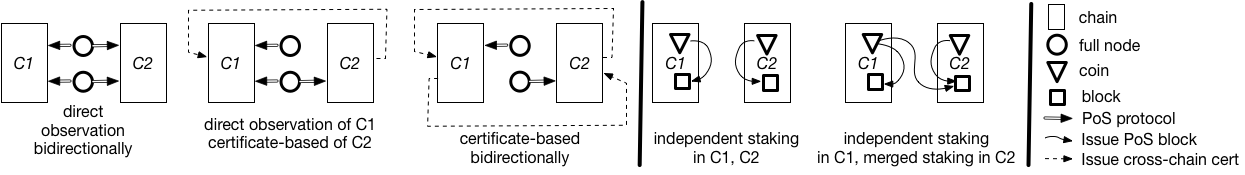
\includegraphics[width=0.95\textwidth]{chapters/sidechains/figures/sidechains-options.png}
  \caption{Deployment options for PoS Sidechains.}
  \label{fig:sidechain-options}
  \end{center}
\end{figure*}

In our construction we choose an exemplary
configuration between two ledgers $\Ledger_1$ and
$\Ledger_2$, so that direct observation is applied to $\Ledger_1$,
cross-chain certification to $\Ledger_2$, independent-staking in $\Ledger_1$ and
merged staking in $\Ledger_2$.
As a result, all stakeholders in $\Ledger_2$ also keep track
of chain development on $\Ledger_1$ (and hence run a full node for $\Ledger_1$)
while the opposite is not necessary, i.e.,
$\Ledger_1$ stakeholders can be oblivious of transactions and
blocks being added to $\Ledger_2$.
This illustrates the two basic possibilities
of pegging and can be easily adapted
to  any other of the configurations between two ledgers in Figure~\ref{fig:sidechain-options}.

In order to reflect the asymmetry between the two chains in our exemplary
construction we will refer to $\Ledger_1$ as the ``mainchain'' $\MC$, and to
$\Ledger_2$ as the ``sidechain'' $\SC$. To elaborate further on this concrete
asymmetric use case, we also fully specify how the sidechain can be
initialized from scratch, assuming that the mainchain already exists.


%We also assume (as discussed in Section~\ref{sec:model}) that all
%actors have relatively synchronized clocks: i.e., clock drift is bounded
%and time can be divided in time slots that all parties can agree on.
%During the existence of the mainchain $\MC$,
%the sidechain can come to existence whenever a new epoch starts on $\MC$.

The pegging with the sidechain will be provided with respect to a specific asset of $\MC$
that will be created on $\MC$.
% PG: not used ever again
%and referred to as the \emph{home} asset of the
%whole sidechain ecosystem.
Note that $\MC$ as well as $\SC$ may carry
additional assets but for simplicity we will assume that staking and pegging is
accomplished only via this single primary asset.

The presentation of the construction is organized as follows. First, in Section~\ref{sec:ats} we introduce a novel
cryptographic primitive, \emph{ad-hoc threshold multisignature (ATMS)}, which is the fundamental building block for cross-chain certification.
Afterwards, in Section~\ref{sec:const} we use it as a black box to build secure
pegged ledgers with respect to concrete instantiations of the functions $\merge$
and $\effect$ and a validity language $\adalang$ for asset~$\ada$ given in Section~\ref{sec:inst}.
Finally, we discuss specific instantiations of ATMS in
Section~\ref{sec:auth}.
